\section{System description and modelling} \label{sec:description}

As described in \cite{rospo}, the ROSPO platform mainly consists in a rigid platform on top of which an arbitrary amount of actuator modules can be mounted. \\
Each of such module is a turret that is able to rotate on it's center with a stepper motor and on top of which a BLDC motor is used to drive propellers that will provide the thrust to move the system. \\
The moving frame is supported by means of omnidirectional passive spherical wheels.

\subsection{Motor modelling}
In contrast to what has been done in the reference paper, this simulation considers a more complex model of the BLDC motor that moves the propeller.

The proposed model is based on the equivalent single coil electrical circuit for the motor that's ruled by the following differential equation:
\begin{equation} \label{eq:singlecoil}
    L \diff{i} t = v - R\, i - e
\end{equation}
where $L, R$ are respectively the inductance and the resistance of the circuit, $i$ is the current flowing, $v$ is the voltage commanded to the circuit and $e$ is the back-electromotive voltage due to the rotation of the motor itself. Called such speed $\Omega$, it holds
\[ \Omega = k_{v} \, e \]

By balancing the electrical power dissipated by the BLDC motor with the resulting mechanical power, the output torque $T_{m}$ of the motor is
\[ T_{m} = \frac{i \, e}{J_{m}} \]
From the body mechanics, the differential equation ruling the angular speed of the rotor is
\begin{equation} \label{eq:rotordyn}
    J_{m} \diff{\Omega}{t} = T_{m} - T_{r}
\end{equation}
where $T_{r}$ is the (positive) resisting torque and $J_{m}$ is the motor's inertia (that comprises also the inertia of the propeller); given that the resisting torque is given just by aerodynamic actions, it can be approximated as $T_{r} = k_{r} \Omega^{2}$.

Combining (\ref{eq:singlecoil}) and (\ref{eq:rotordyn}) and removing the different algebraic constraints, leads to the following system of ODEs ruling the behavior of the BLDC motor:
\begin{equation} \label{eq:motordynamics}
\begin{cases}
    L \diff{i} t & = v - R \, i - \frac{\Omega}{k_{v}} \\
    J_{m} \diff{\Omega}t & = \frac{i}{k_{v}} - k_{r} \Omega^{2}
\end{cases}
\end{equation}
where $\Omega, i$ are the states of the system and $v$ is the input. Finally the force of the propeller $F_{p}$ is given by the state simply as
\begin{equation} \label{eq:motorforce}
    F_{p} = k_{l} \Omega^{2}
\end{equation}
where $k_{l}$ is the lift coefficient.

Numerically, all constants have been obtained, whenever possible, directly from datasheet of propellers and motors present in the laboratories; when data were not available, they have been derived considering simple mechanics. Table \ref{tab:motorcoeffs} report all such values.
\begin{table}[bt]
    \centering
    \caption{coefficients used in the motor's model.}
    \label{tab:motorcoeffs}
    \begin{tabular}{c c}
        constant & value \\ \hline \hline
        $k_{v}$ & $750 V / rpm$ \\
        $L$ & $27.2mH$ \\
        $R$ & $0.7 \Omega$ \\
        $k_{l}$ & $6.4\cdot 10^{-4}$ \\
        $k_{r}$ & $1.2\cdot 10^{-5}$ \\
        $J_{m}$ & $2.8\cdot 10^{-4} kg\cdot m^{2}$ \\
    \end{tabular}

\end{table}




\subsection{Friction force}
The reference model embeds also the effects of friction forces on the spherical wheels; the continuous function used is based on \cite{friction} and is of the form
\begin{equation} \label{eq:fricforce}
    \vett F_{f,\vett p}(\vett v) =
    \begin{cases}
        \mu(|\vett v|) \frac{\vett v}{|\vett v|} & \vett v \neq 0 \\
        0 & v = 0
    \end{cases}
\end{equation}
where $\vett v \in \mathbb R^{2}$ is the velocity of the point $\vett p$ in the plane and $\mu$ is the continuous function defined as
\[ \mu(s) = \gamma_{1}\big(\tanh(\gamma_{2}s) - \tanh(\gamma_{3} s)\big) + \gamma_{4} \tanh(\gamma_{5}s) + \gamma_{6} s \]

In the provided model $\gamma_{1}, \gamma_{2}, \gamma_{3}, \gamma_{6}$ are set to zero to neglect both Stribeck effect and viscous dissipation.
Since (\ref{eq:fricforce}) is continuous, it's time derivative later used in the control law can be computed as
\begin{equation} \label{eq:fricderivative}
    \dvett F_{r,\vett p}(\vett v) = \left(
        \left( \matt I  - \frac{\vett v \vett v^{\top}}{\vett v^{\top} \vett v} \right) \mu \big(|\vett v|\big)
        + \frac{\vett v \vett v^{\top}}{|\vett v|}\mu'\big(|\vett v|\big)
    \right) \frac{\dvett v}{|\vett v|}
\end{equation}
with
\begin{equation} \label{eq:mudt}
    \mu'(s) = \gamma_{4}\big(1 - \tanh^{2}(\gamma_{5}s) \big) \gamma_{5}
\end{equation}


\subsection{ROSPO modelling}
\begin{figure}[bt]
    \centering
    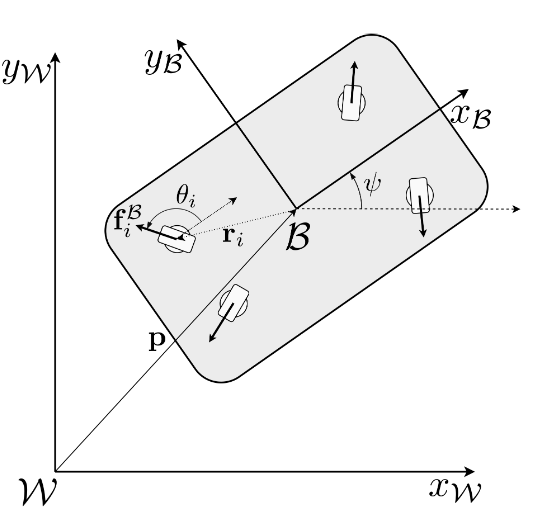
\includegraphics[width=5cm]{Images/rospo-scheme}
    \caption{schematic illustration of the ROSPO system; image courtesy of \cite{rospo}.}
    \label{fig:scheme}
\end{figure}
The ROSPO system is described as a single rigid body, i.e. the changes in mass and inertias due to the turrets rotations have been disregarded.
With this approximation in place the system's dynamic is described as
\begin{equation} \label{eq:dynamics}
\begin{cases}
    m \ddvett p_{com} & = \matt R(\psi)\sum_{i} F_{p,i} \vers u(\phi_{i}) + \sum_{i} \vett F_{r, \vett p_{i}} \\
    J \ddot \psi & = \sum_{i} \vett r_{i} \times F_{p,i} \vers u(\phi_{i}) + \sum_{i} \vett r_{\vett p_{i}} \times \vett F_{r, \vett p_{i}} \\
    \dot \phi_{i} & = \delta_{i}
\end{cases}
\end{equation}
where $\vers u(\phi_{i}) = \big(\cos(\phi_{i}), \sin(\phi_{i})\big)^{\top}$ represents the direction where the force $F_{p,i}$ of the $i$-th propeller is applied, with $\phi_{i}$ the relative orientation of the turret w.r.t the body's local frame that's described by an orientation $\psi$; $\vett r_{\circ}$ are instead the vectors describing the distance of the point where the force is applied w.r.t. the center of mass of the ROSPO; finally $m,J$ are the mass and the inertia of the system. \\
The rotation matrix \[ \matt R(\psi) = \begin{bmatrix} \cos \psi & -\sin\psi \\ \sin\psi & \cos\psi \end{bmatrix} \]
is used to convert the force computed in the local frame of the body into the inertial ground reference frame. \\
The dynamics of the turret's attitude $\phi_{i}$ is linear w.r.t. the corresponding input $\delta_{i}$ since such element is moved by a stepper motor.

After reducing the system to a first order ODE the states $\vett x$ and input $\vett u$ are:
\begin{equation} \label{eq:states}
\vett x =
\begin{pmatrix}
    x_{com} \\ y_{com} \\ \psi \\ v_{x,com} \\ v_{y, com} \\ \omega \\
    \Omega_{1} \\ i_{1} \\ \phi_{1} \\ \vdots \\ i_{N_{t}} \\ \phi_{N_{t}}
\end{pmatrix} \in \mathbb R^{6 + 3N_{t}}
\qquad \vett u =
\begin{pmatrix}
    v_{1} \\ \delta_{1} \\ \vdots \\ v_{N_{t}} \\ \delta_{N_{t}}
\end{pmatrix} \in \mathbb R^{2N_{t}}
\end{equation}
where $N_{t}$ is the number of turrets installed on the ROSPO platform that for the following simulation is chosen to $4$.

